\documentclass[12pt]{sciposter}
%[portrait]
%\documentclass[xcolor={table}]{beamer}
%\documentclass[a4paper]{article}
\usepackage[utf8]{inputenc}
\usepackage[spanish]{babel}
\usepackage{url}
\usepackage{amsmath}
\usepackage{amsfonts}
\usepackage{amssymb}
\usepackage{verbatim}
%\usepackage{ngerman}
\usepackage{graphicx}
%\usepackage[pdftex]{color}
%\usepackage{subfigure}
\usepackage{multicol}
\usepackage{sectionbox}
\newtheorem{defi}{Definición}


\author{Daniel Calvo Briceño}
%\addauthor[mail,diam]{J.F. Nash}
\title{ \begin{Huge} 
Análisis espacial de la incidencia de cáncer de piel, mama y próstata en Costa Rica
\end{Huge}
}
\institute{Universidad de Costa Rica\\}
\email{daniel.calvobriceno@ucr.ac.cr, \ github.com/danielcalvo27 } 
%\leftlogo[1]{UniLogo2}
%\rightlogo[1]{TEM-Logo}
\conference{Curso de Estadística Espacial. Maestría de Estadística, 2020}
\begin{document}

\maketitle
\\
\rule{\textwidth}{2mm}

\begin{multicols}{2}

\begin{abstract}
El cáncer de piel, mama y próstata corresponden a los tipos de tumores malignos más frecuentes a nivel nacional. Los dos últimos tienen el primer lugar de mortalidad para hombres y mujeres respectivamente, por lo cual, son de monitoreo constante para las autoridades de salud. Este estudio parte de la información del 2014, suministrada por el Registro Nacional de Tumores del Ministerio de Salud, donde se obtiene la cantidad de casos y el tipo cáncer por cantón, sexo o edad. Esta información será analizada mediante las técnicas de estadística espacial, para identificar clúster, patrones y relaciones entre las incidencia y mortalidad de estos tipos de cáncer
\bigskip


\end{abstract}

\section{Introducción}

El cáncer de piel, mama y próstata corresponden a los tipos de tumores malignos más frecuentes a nivel nacional. El cáncer de piel fue el de la mayor incidencia (diagnóstico) para el sexo masculino en el 2014 y el segundo más frecuente para mujeres en el mismo año. En este estudio se realizará un análisis geo espacial descriptivo de la ubicación donde se presenta la mayor incidencia de estos tipos de cáncer. Aunado a esto se agregará al análisis espacial la mortalidad por cáncer de mama y próstata que corresponden al primer lugar en este rubro para el sexo femenino y masculino. En el caso del cáncer de piel a pesar de que su frecuencia en incidencia es alta, no está dentro de los tumores con mayor frecuencia de mortalidad. La ubicación espacial se realizará nivel de cantón y responderá la pregunta de si existen focos para la incidencia y mortalidad de estas patologías. 
 
\bigskip

Según las estadísticas del Ministerio de Salud desde el año 2000, el cáncer de piel y el mama para el sexo femenino se han mantenido como los de mayor incidencia ambos por encima de una tasa de incidencia de 40 mujeres por cada 100.000. Antes del 2005 inclusive, el cáncer con mayor incidencia era el Cérvix, llegando a tener una disminución cercana al $33\%$ del 2000 al 2012, esta disminución corresponde a una fuerte inversión por parte de las autoridades de Salud en equipo médico especializado y a las campañas de auto cuidado (véase figura \ref{fig_inc_CCSS}). En el caso de la mortalidad el cáncer de mama, posee la mayor frecuencia desde el año 2000, con tasas superiores de 10 mujeres por cada 100.000.

\bigskip

\begin{figure}[h]
\begin{center}
\label{fig_inc_CCSS}
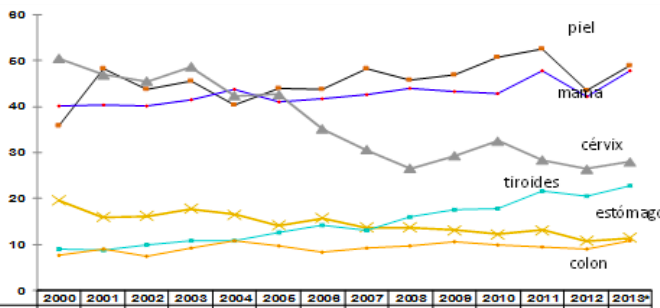
\includegraphics[width=\textwidth]{inc_CCSS1.png}
\caption{Incidencia por tumores malignos más frecuentes en las mujeres según año. Fuente: Ministerio de Salud \cite{Salud} }
\end{center}
\end{figure}

En el caso de los hombres, los datos recientes muestran como al cáncer de piel y próstata como los de mayor incidencia desde el año 2000, con tasas de incidencias significativamente mayores al resto, aunado a la baja que ha presentado el cáncer de estomago desde el año 2000. (veáse figura  \ref{fig_inc_CCSS2}).

\begin{figure}[h]
\begin{center}
\label{fig_inc_CCSS2}
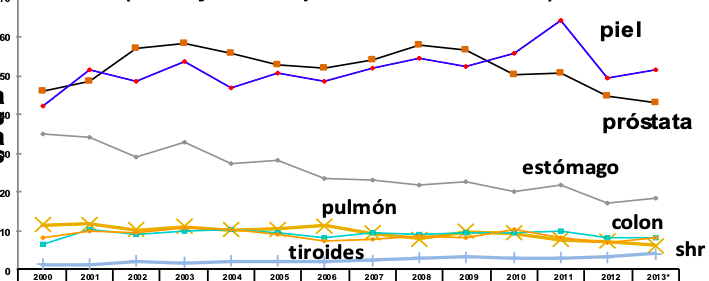
\includegraphics[width=\textwidth]{inc_CCSS2.png}
\caption{Incidencia por tumores malignos más frecuentes en las hombres según año. Fuente: Ministerio de Salud \cite{Salud} }
\end{center}
\end{figure}

La información utilizada procede del Ministerio de Salud de dos distintas fuentes. En primer lugar la información de incidencia y mortalidad por género se extrajo del Registro Nacional de tumores, donde esta información se presenta por cantón, e incluye la tasas de incidencia y mortalidad por cada $100.000$ habitantes  \cite{Salud}. Adicional a esto, los mapas de la distribución cantonal de Costa Rica se descargaron del Observatorio Geográfico de Salud \cite{OGES}.


\section{Problema de investigación}

Realizar un análisis espacial sobre la distribución de la incidencia y mortalidad para los cáncer de mayor frecuencia en Costa Rica por hombres y mujeres, con el objetivo de estudiar su localización y determinar clúster o patrones a nivel nacional.

\section{Datos}

Los datos para obtener la incidencia del cáncer de piel, mama y próstata en Costa Rica fueron extraídos de la página del Ministerio de salud, del registro nacional de tumores \cite{Salud}. Este centro registra desde 1976 los caso de tumor maligno que se diagnostican en Costa Rica, gracias a la declaración del cáncer como enfermendad de notificación obligatoria. Los registros de los casos se realizan mediante los estándares de la Agencia Internacional de Investigación en Cáncer (IARC por sus siglas en inglés). La información utilizada es del año 2014 que fue la más reciente obtenida para la incidencia y la mortalidad en un mismo año. La georeferencia se obtuvo del Observatorio Geográfico de Salud \cite{OGES}. El archivo de datos es del tipo \verb|shp|, la base contiene un total de 81 observaciones y 4 variables. Estas son cantón, provincia, incidencia y la geometría del cantón que del tipo \textit{polígono} y con la proyección \verb|WGS84|. 
\bigskip

\begin{defi}
La incidencia de un tipo de cáncer, es el número de casos nuevos que se registran en una población en un período de tiempo y en un lugar determinado \cite{OGES}.
\end{defi}
\bigskip

El cuadro 1, muestra la incidencia del cáncer de piel el más frecuente en Costa Rica, por cantón y sexo y el mapa de la figura 3, se puede este indicador a nivel nacional.
\bigskip

\begin{table}[t]
\begin{center}
\begin{tabular}{llll}
Cantón   & Tasa Total    & Tasa Hombres & Tasa Mujeres \\ \hline
Puriscal & 195       & 165     & 227        \\
San Mateo   & 149     & 144        & 155          \\
Pérez Zeledon & 120 & 107 & 133                                      \\
San José      & 112 & 116 & 108                                      \\
Montes de Oro    & 112    & 104       & 120     \\   \hline   
\end{tabular}
\caption{Incidencia cantonal por cada 100 mil habitantes del cáncer de piel. Fuente: \cite{Salud} }
\label{tabla1}
\end{center}
\end{table}

Dado que el indicador de incidencia está asociado a la cantidad de población en el cantón, una variable adicional que se está considerando agregar al análisis es la tasa de incidencia y mortalidad para la población mayor de 40 años podría llegar a generar valor agregado por los tipos de cáncer que se consideran el análisis.
\bigskip

\begin{figure}[h]
\begin{center}
\label{can_piel}
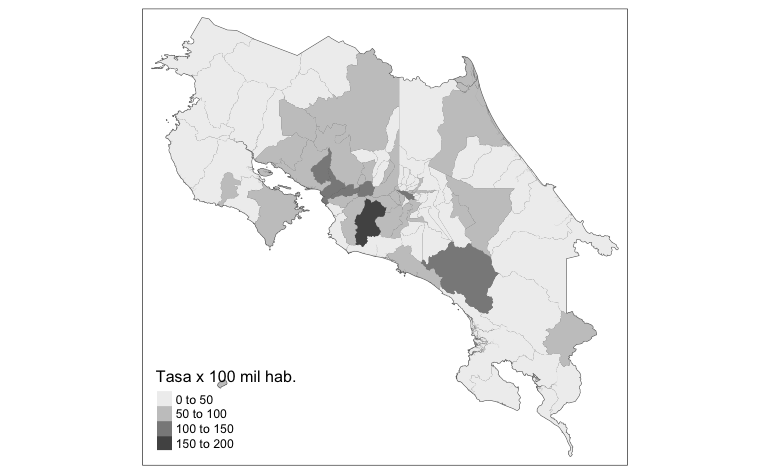
\includegraphics[scale=1.55]{graf3.png}
\caption{Distribución cantonal de la tasa de incidencia de cáncer de piel}
\end{center}
\end{figure}


%\begin{figure}[h]
%\begin{center}
%\label{fig_twin}
%\includegraphics[width=\textwidth]{poster_aperture_twin.png}
%\end{center}
%\caption{setup -- twin aperture}
%\end{figure}
% one electron wave is shifted in phase such that the phase difference of the two waves in the sample plane is $\pi/2$ and such that a similar diffraction pattern is observed in the diffraction plane as for the intrinsic method. 

%Therefor the possibility of a STEM operation with such a twin aperture was investigated due to the wish to perform EMCD measurement in a STEM mode in the future.



%\textbf{\scshape Intensity Distribution}: $|\psi_{BFP}|^2$, see fig. %\ref{fig_linescan}


%\begin{figure}[h]
%\includegraphics[width=\textwidth]{poster_linescan.png}
%\caption{intensity distribution and phase difference}
%\label{fig_linescan}
%\end{figure}



%\textbf{\scshape Definition}: quality parameter $U$ and weighting function $\Upsilon$:
%\begin{eqnarray}
%\label{eqn_usignal}
%U &=& \frac{\int\limits_{-\infty}^\infty\Upsilon(X)|\psi_{BFP}(X,\,0)|^2\,\mathrm{d}X}{\int\limits_{-\infty}^\infty|\psi_{BFP}(X,\,0)|^2\,\mathrm{d}X} \nonumber\\
%\label{eqn_upsilon_1}
%\Upsilon(X) &=& 2\,\mathrm{sgn}\left(\Delta\phi(X)\right)\left|\left(\frac{\Delta\phi(X)}{\pi}+\frac{1}{2}\right)\mathrm{mod}\,1-\frac{1}{2}\right| %\nonumber\\
%\label{eqn_sn}
%\mathrm{S/N} &=& \frac{\int\limits_a^b|\psi_{BFP}(X,\,0)|^2\,\mathrm{d}X}{\int\limits_{-\infty}^\infty|\psi_{BFP}(X,\,0)|^2\,\mathrm{d}X},\;[a,\,b]: \mathrm{FWHM} \nonumber
%\end{eqnarray}



%\begin{figure}[h]
%\begin{center}
%\includegraphics[width=\textwidth]{poster_upsilon.png} 
%\end{center}
%\caption{weighting function $\Upsilon$ (for legend see fig. \ref{fig_linescan})}
%\label{fig_upsilon}
%\end{figure}



%\begin{figure}[hbt]
%\label{fig_sql_1}
%\includegraphics[width=.8\textwidth]{poster_sql_u.png}
%\includegraphics[width=\textwidth]{poster_usignal_2.png}
%\caption{evaluation -- $U$}
%\end{figure}

%\begin{figure}[hbt]
%\includegraphics[width=.8\textwidth]{poster_sql_sn.png}
%\includegraphics[width=\textwidth]{poster_sn_2.png}
%\caption{evaluation -- Signal/Noise (for legend see fig. \ref{fig_sql_1})}
%\label{fig_sql_2}
%\end{figure}




%\begin{figure}[hbt]
%\label{fig_goldstem}
%\subfigure[twin aperture]{\label{fig_goldstem_a}
%\includegraphics[width=.475\textwidth]{gold_einzel_50k.png}
%\includegraphics[width=.45\textwidth]{8061-5png.png}}
%\subfigure[STEM image]{\label{fig_goldstem_b}\includegraphics[width=.45\textwidth]{gold_twin_50k.png}}
%\caption{twin aperture (w/o phase plate) \& STEM image of gold particles using twin aperture.}
%\end{figure}

%Figure \ref{fig_goldstem} shows images observed in STEM-mode with the CM30 




\begin{thebibliography}{0}

  \bibitem{Salud} Ministerio de Salud, Dirección Vigilancia de la Salud, Unidad de Seguimiento de Indicadores de Salud, Registro Nacional de Tumores.
  
  \bibitem{OGES} Observatorio Geográfico en Salud. Ministerio de Salud Costa Rica.
  \url{http://geovision.uned.ac.cr/oges}
  
\end{thebibliography}





\end{document}
      
      
      
      
      